% Appendix A

\chapter{Appendix Title Here} % Main appendix title

\label{AppendixA} % For referencing this appendix elsewhere, use \ref{AppendixA}

\lhead{Appendix A. \emph{Appendix Title Here}} % This is for the header on each page - perhaps a shortened title

\begin{figure}[h]
\centering
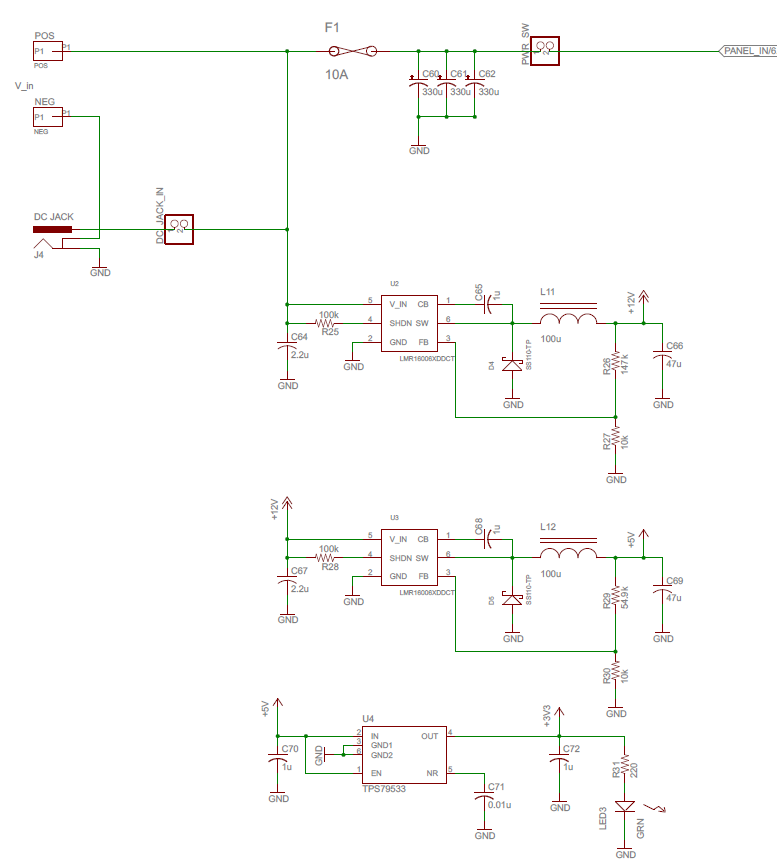
\includegraphics[width = 3.5in]{logic_power.PNG}
\caption{Logic Power Supply Circuit}
\label{logic power fig}
\end{figure}


\begin{figure}[h]
\centering
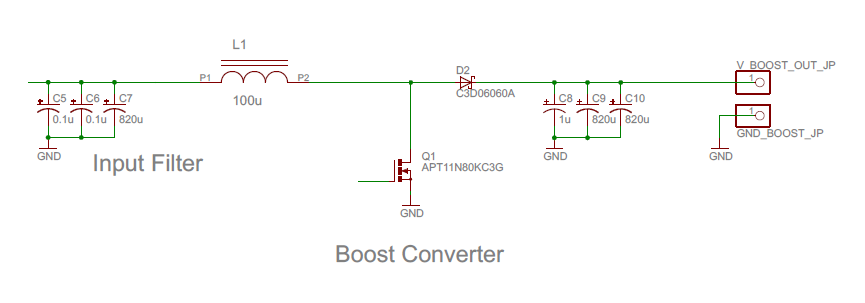
\includegraphics[width = 3.5in]{sch_boost.png}
\caption{Boost Converter Circuit}
\label{boostConverterCircuit}
\end{figure}

\begin{figure}[h]
\centering
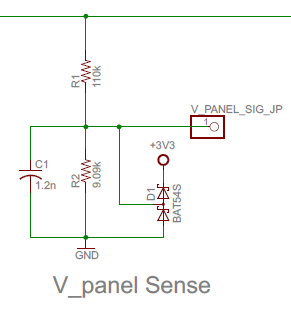
\includegraphics[width = 3.5in]{sch_Vpanel.png}
\caption{PV Voltage Sense Circuit}
\label{VpvSenseCircuit}
\end{figure}

\begin{figure}[h]
\centering
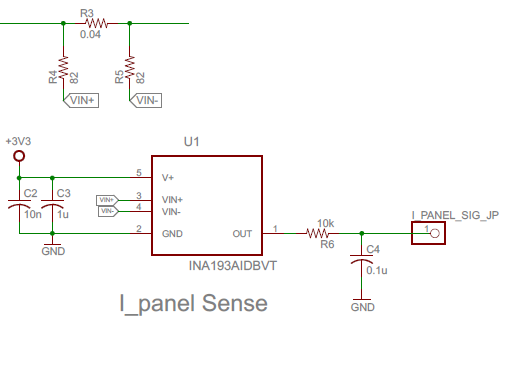
\includegraphics[width = 3.5in]{sch_Ipanel.png}
\caption{PV Current Sense Circuit}
\label{IpvSenseCircuit}
\end{figure}

\begin{figure}[h]
\centering
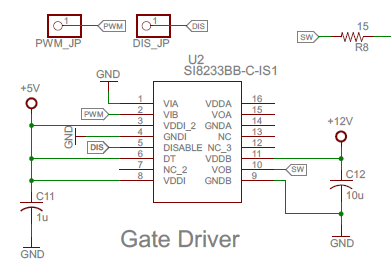
\includegraphics[width = 3.5in]{sch_driver.png}
\caption{ Gate Driver Circuit}
\label{gateDriverCircuit}
\end{figure}

\begin{figure}[h]
\centering
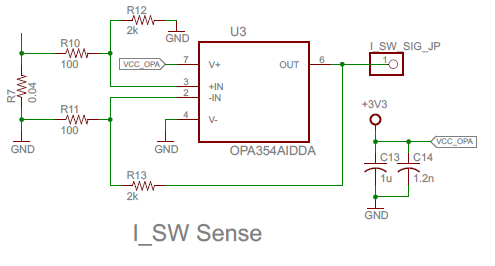
\includegraphics[width = 3.5in]{sch_Isw.png}
\caption{Switch Current Sense Circuit}
\label{IswSenseCircuit}
\end{figure}

\begin{figure}[h]
\centering
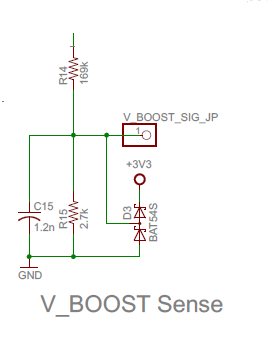
\includegraphics[width = 3.5in]{sch_Vboost.png}
\caption{Boosted Voltage Sense Circuit}
\label{VboostSenseCircuit}
\end{figure}

\begin{figure}[h]
\centering
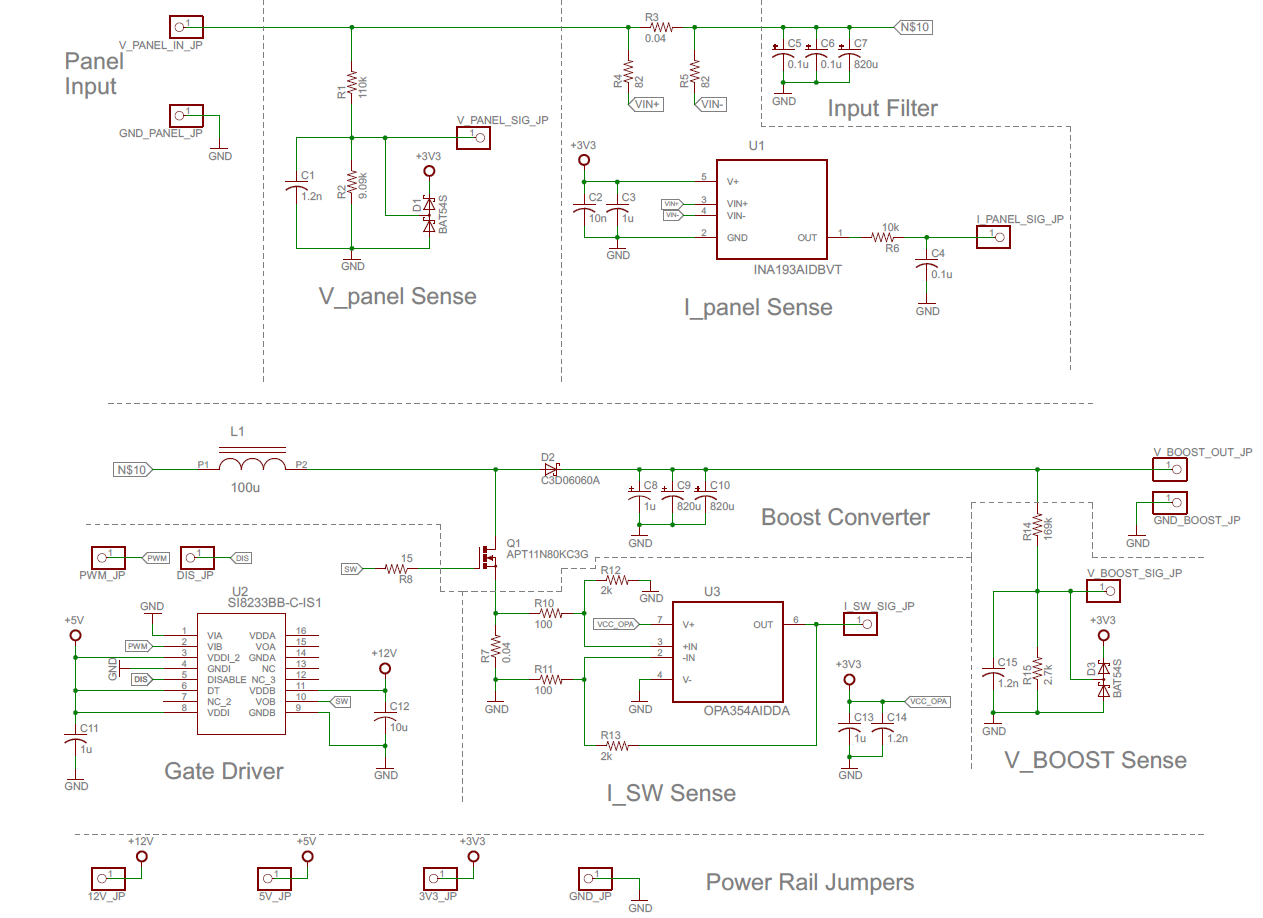
\includegraphics[width = 3.5in]{Boost_Schematic.PNG}
\caption{Boost Converter Schematic}
\label{boostCompleteSchematic}
\end{figure}

\begin{figure}[h]
\centering
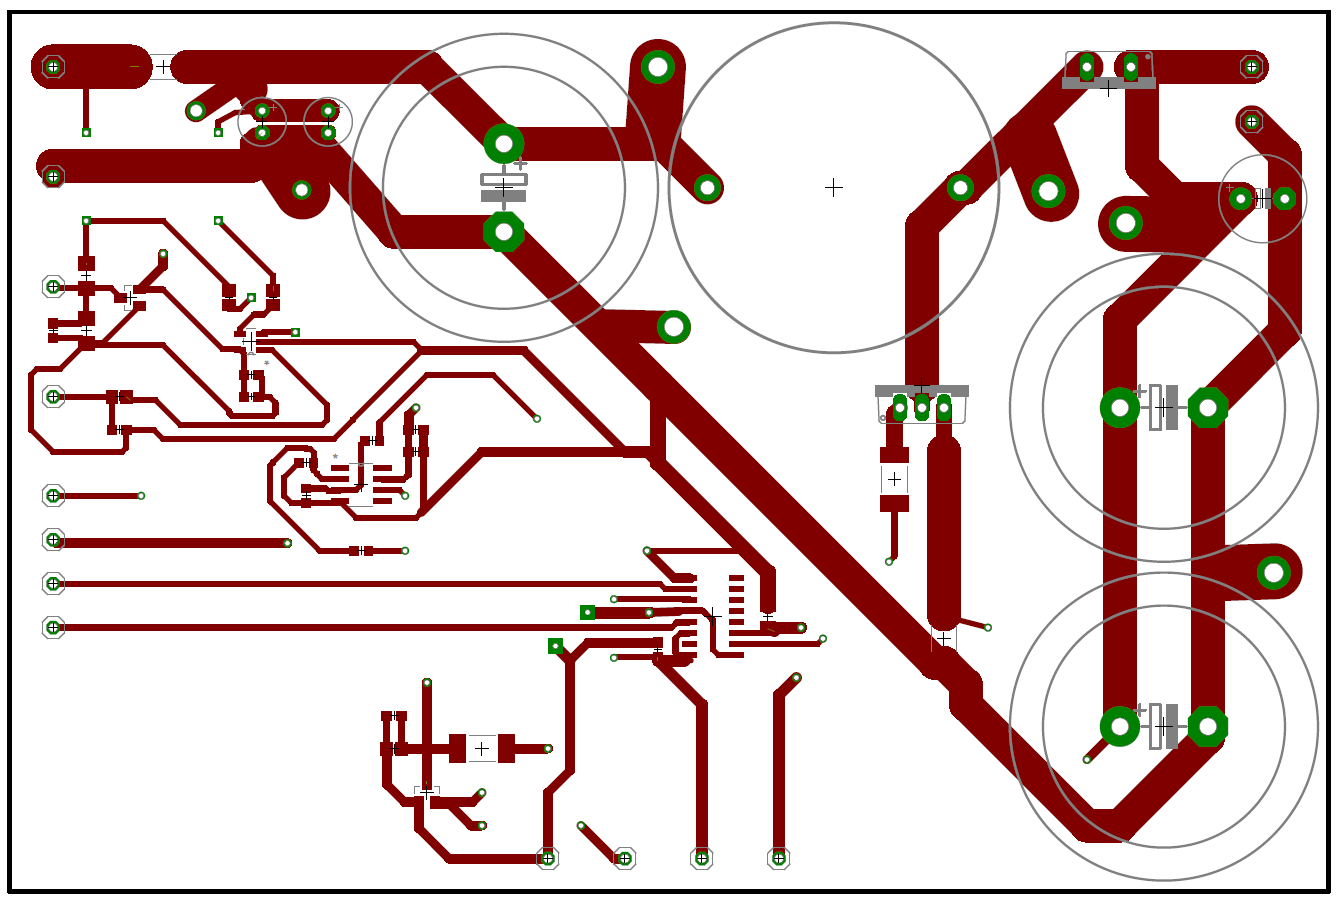
\includegraphics[width = 3.5 in]{Boost_PCB_TOP.PNG}
\caption{Boost Board PCB Top}
\label{boostPCBTop}
\end{figure}

\begin{figure}[h]
\centering
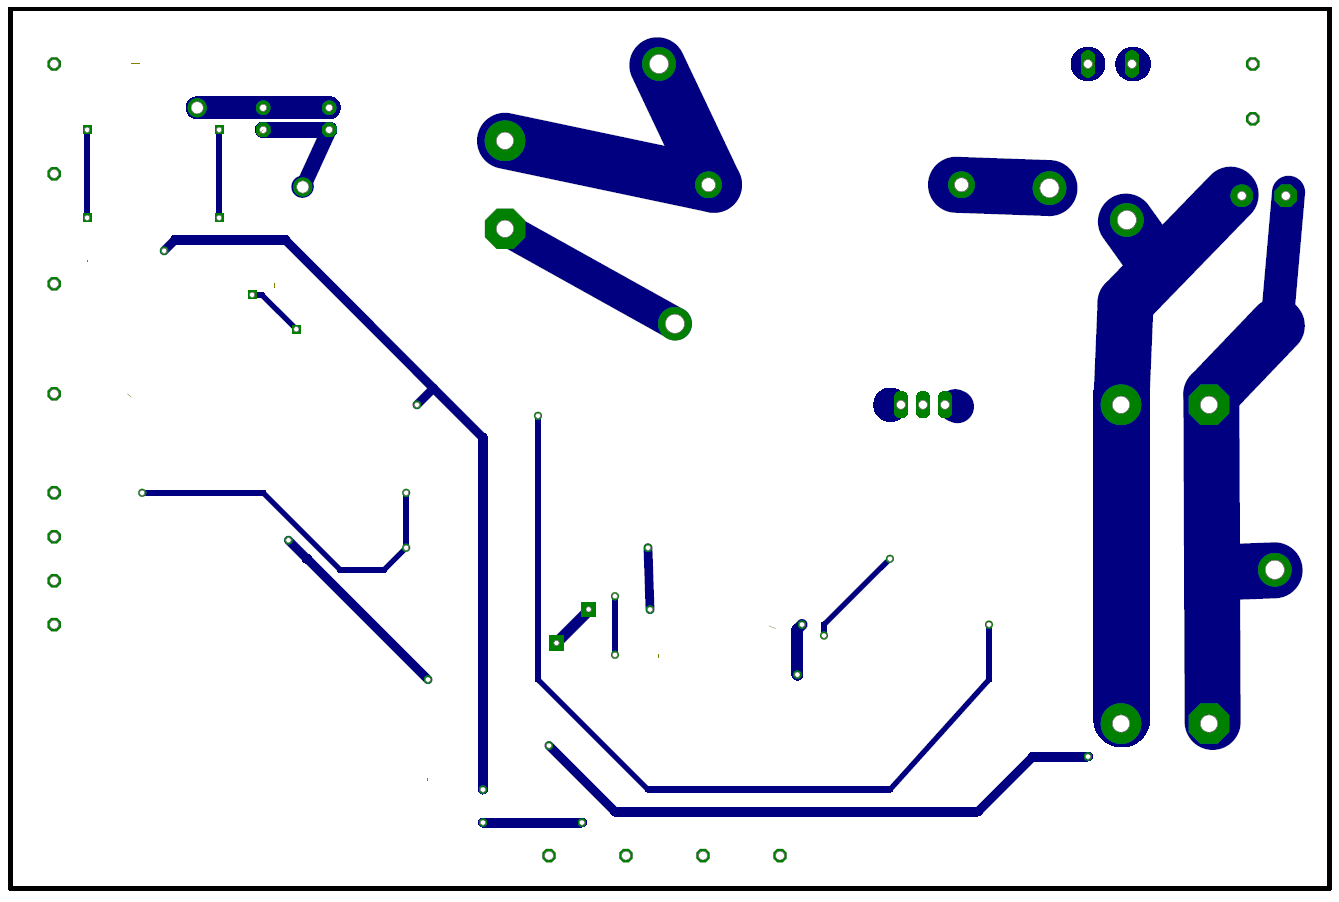
\includegraphics[width = 3.5 in]{Boost_PCB_BOTTOM.PNG}
\caption{Boost Board PCB Bottom}
\label{boostPCBBottom}
\end{figure}

\begin{figure}[h]
\centering
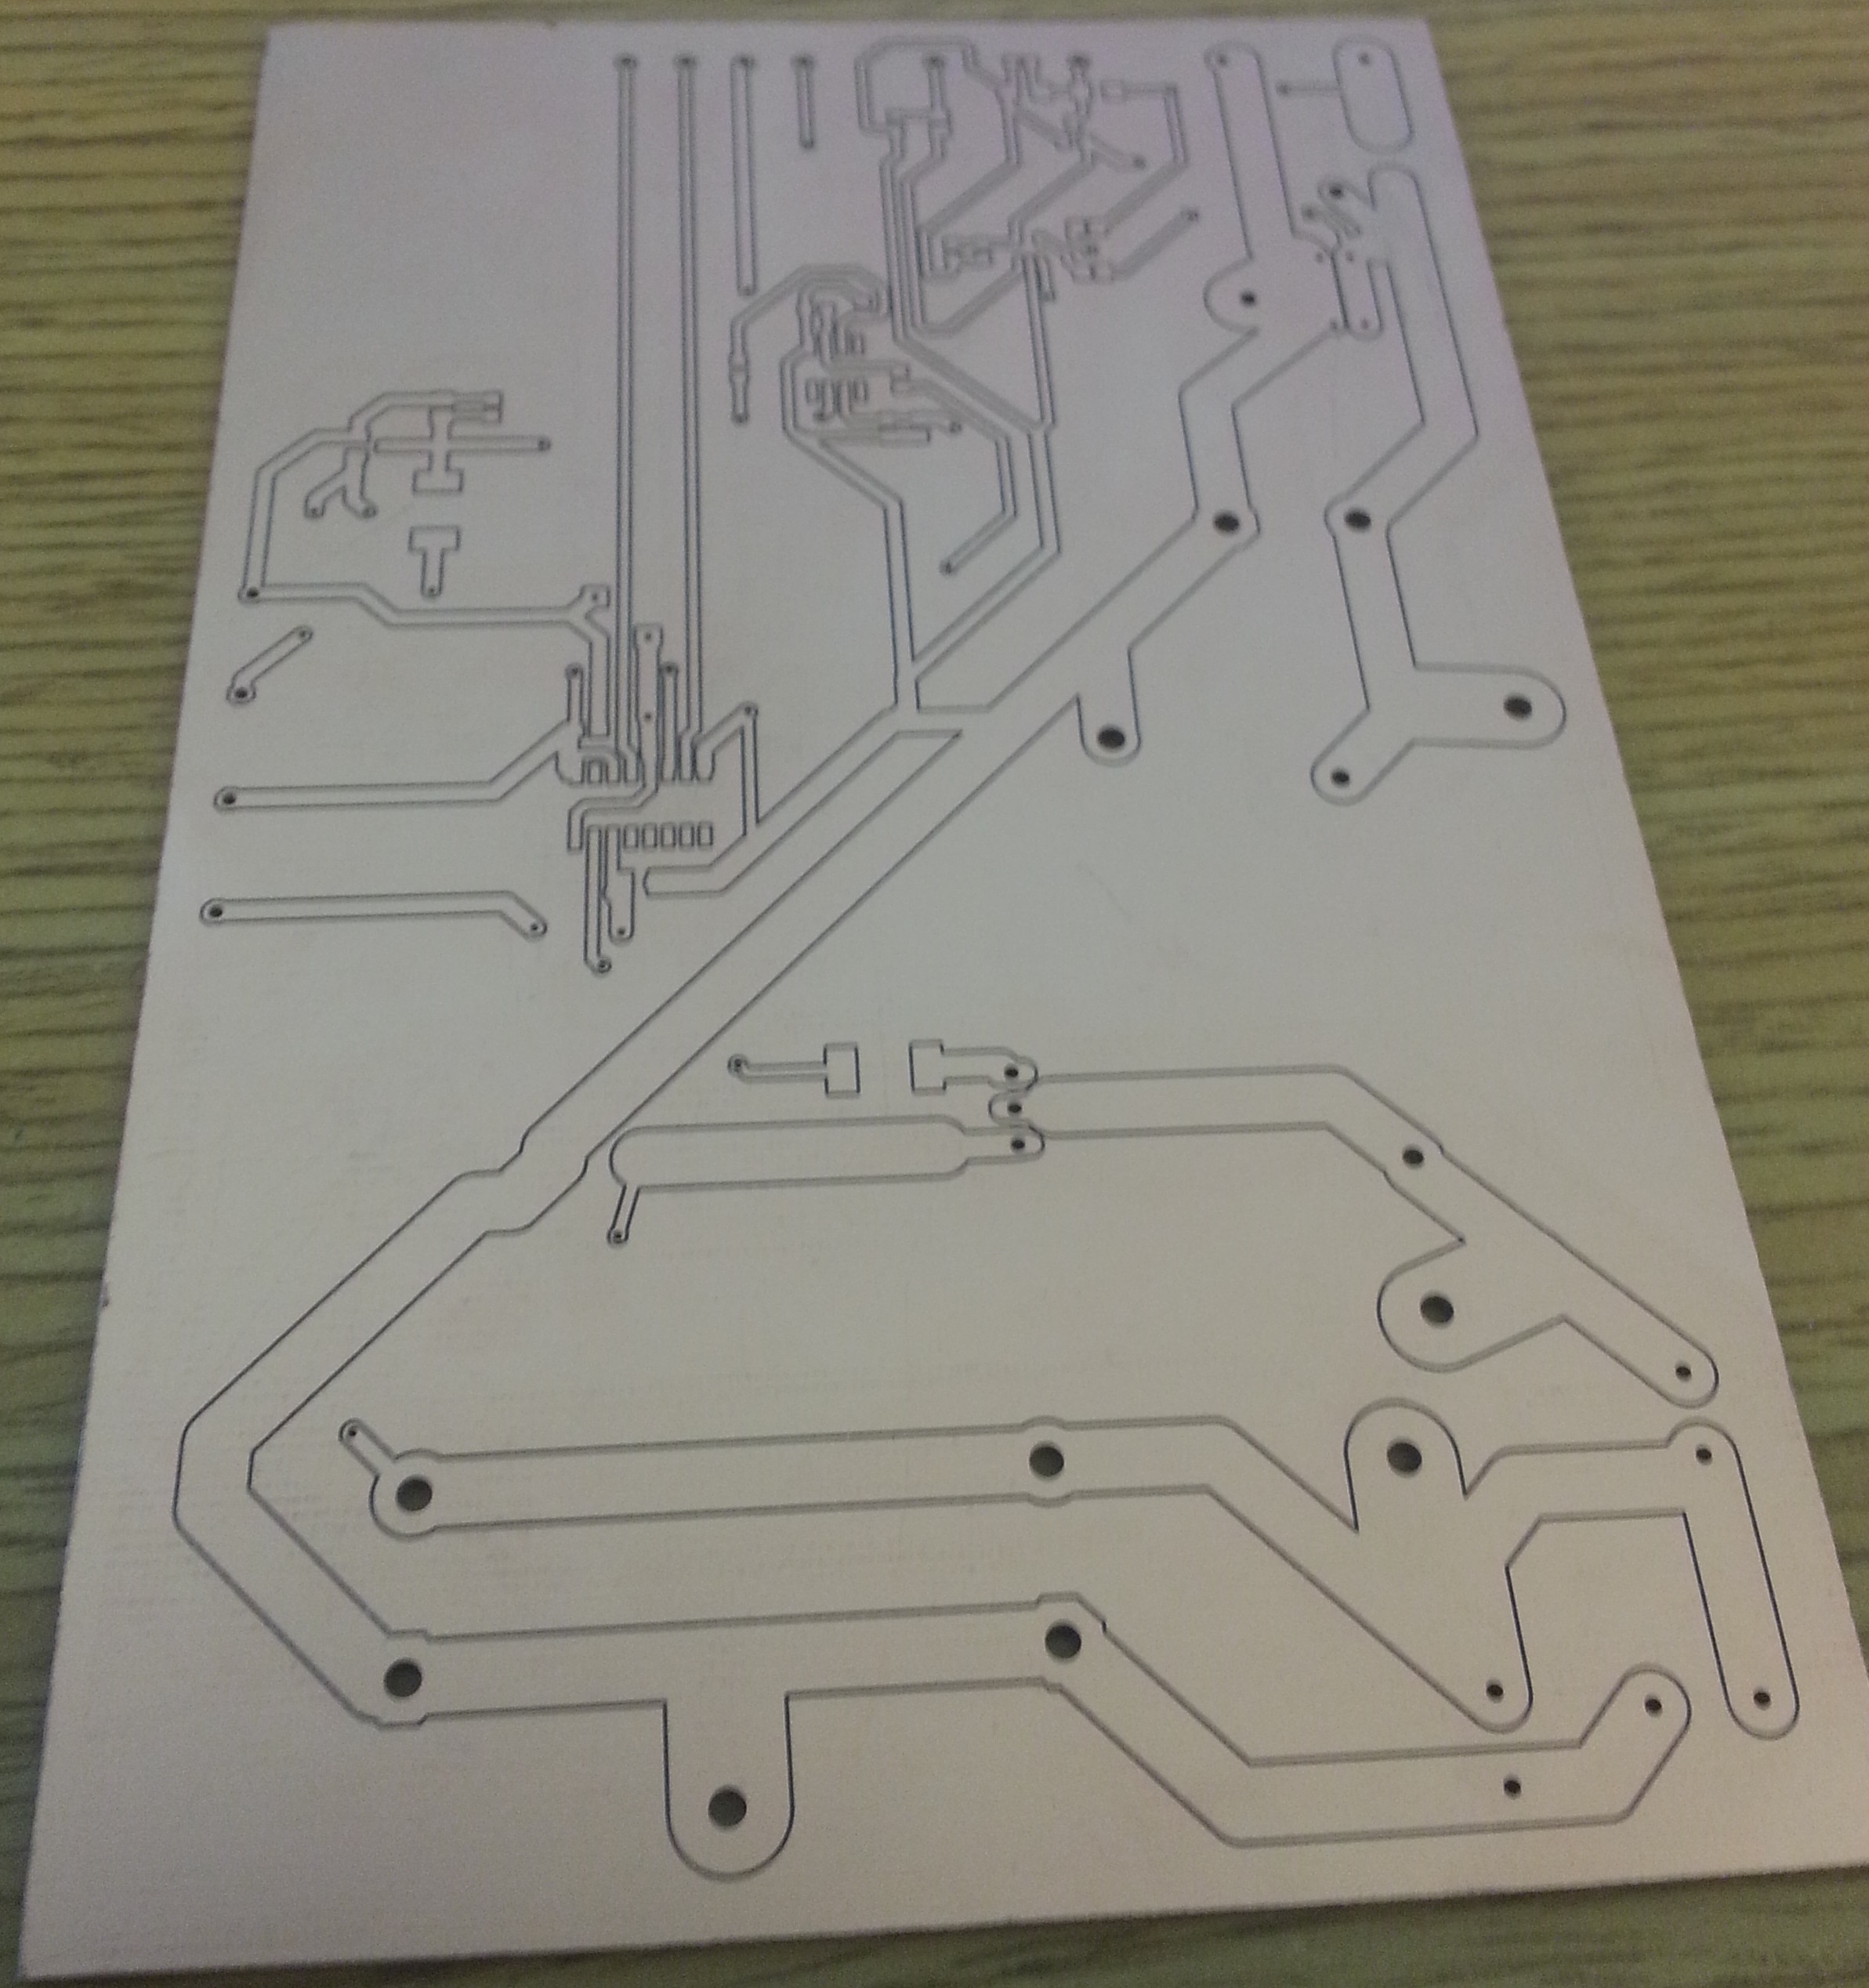
\includegraphics[width = 3.5in]{boost_PCB_routed.jpg}
\caption{Board Board PCB}
\label{unpopulatedBoostPCB}
\end{figure}

\begin{figure}[h]
\centering
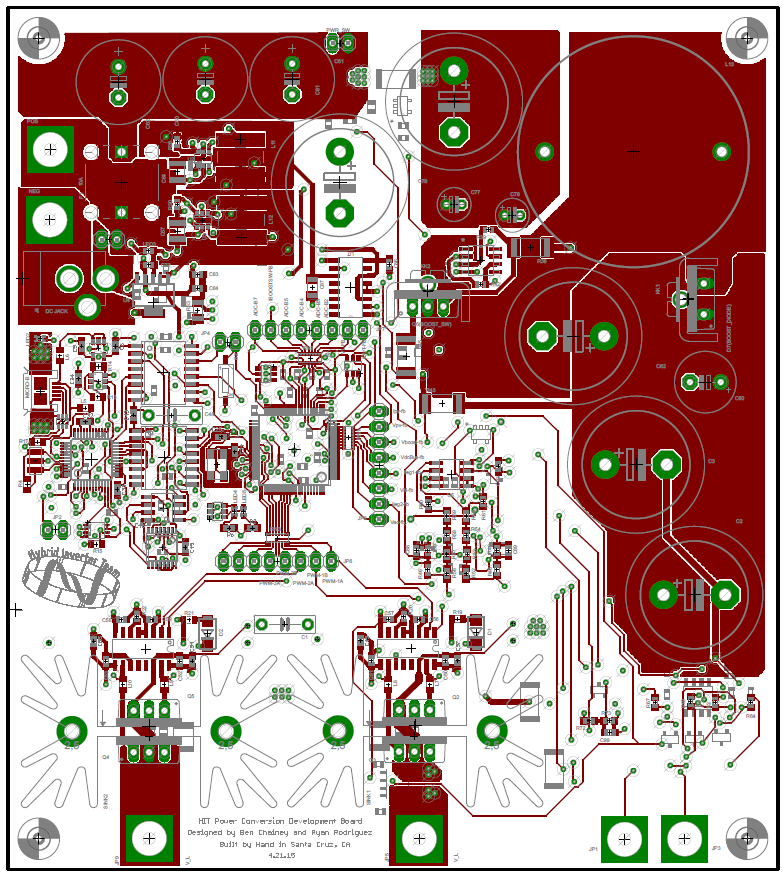
\includegraphics[width = 3.5in]{PCB_top.PNG}
\caption{PCB Top Layer}
\label{PCB top}
\end{figure}

\begin{figure}[h]
\centering
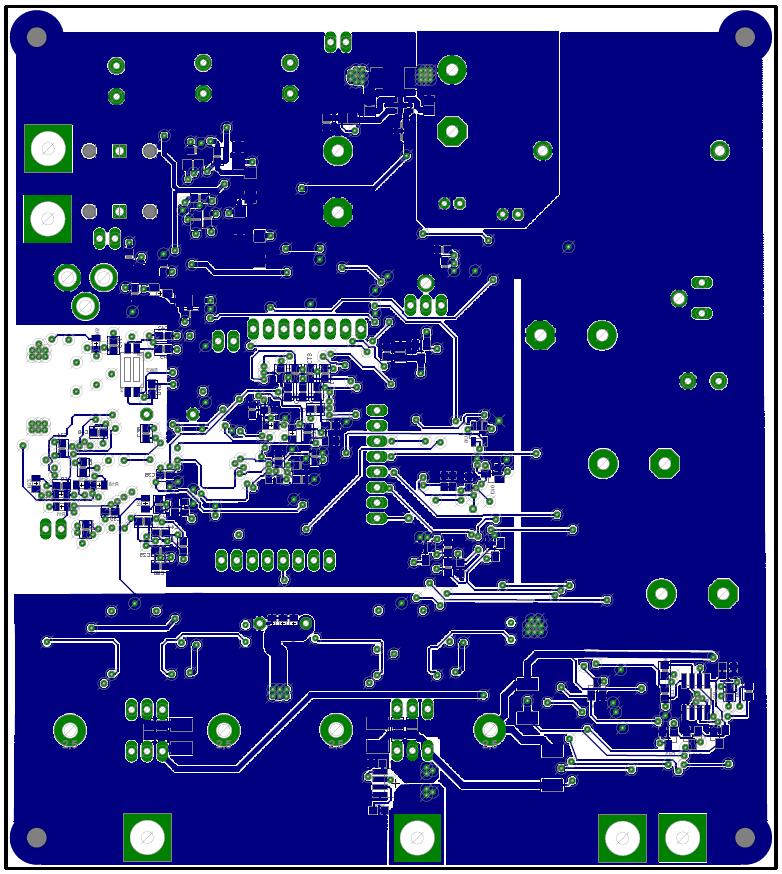
\includegraphics[width = 3.5in]{PCB_bottom.PNG}
\caption{PCB bottom}
\label{PCB bottom}
\end{figure}